\subsection{Single Source for Office datasets}
There are 3 subsets in offices datasets, webcam (795), amazon (2817) and dslr (498), sharing 31 classes. We perform 2 adaptation experiments, transferring from webcam to amazon and from dslr to amazon. 

We use the features extracted from Alexnet \cite{KrizhevskyNIPS12} FC7 as the input features for both source and target domain. The teacher (source) model is trained with MLP on the whole source dataset and student (target) model is trained with GDDA-SVM. We also use brute force to search the imitation parameter $\lambda$ in range $[0,0.1,...,1]$ and show the results. Here our experiments run in a semi-supervised scenario where there are some unlabeled data in the target training set in each experiment. We also show the performance of the teacher model on the target task, denoted as "teacher". To avoid the randomness, we perform each experiments 10 times and report the results. The experiment results are shown in Figure \ref{fig:single1} and \ref{fig:single2} respectively.

\textbf{Observation:} The performance of the target model can exceed the performance of the teacher in a "one-short" learning scenario. This means the target model can quickly learn the knowledge of the teacher. \hl{Increasing the size of the unlabeled example doesn't necessarily increase the performance. The performance of the model increases at the beginning but decreases then. May due to the performance of the difference between the source model and target model.}
%\newpage
%\subsubsection{From DSLR to Amazon}
\begin{figure}[h]
\centering
\begin{tabular}{cc}
\subfloat[5 unlabeled ]{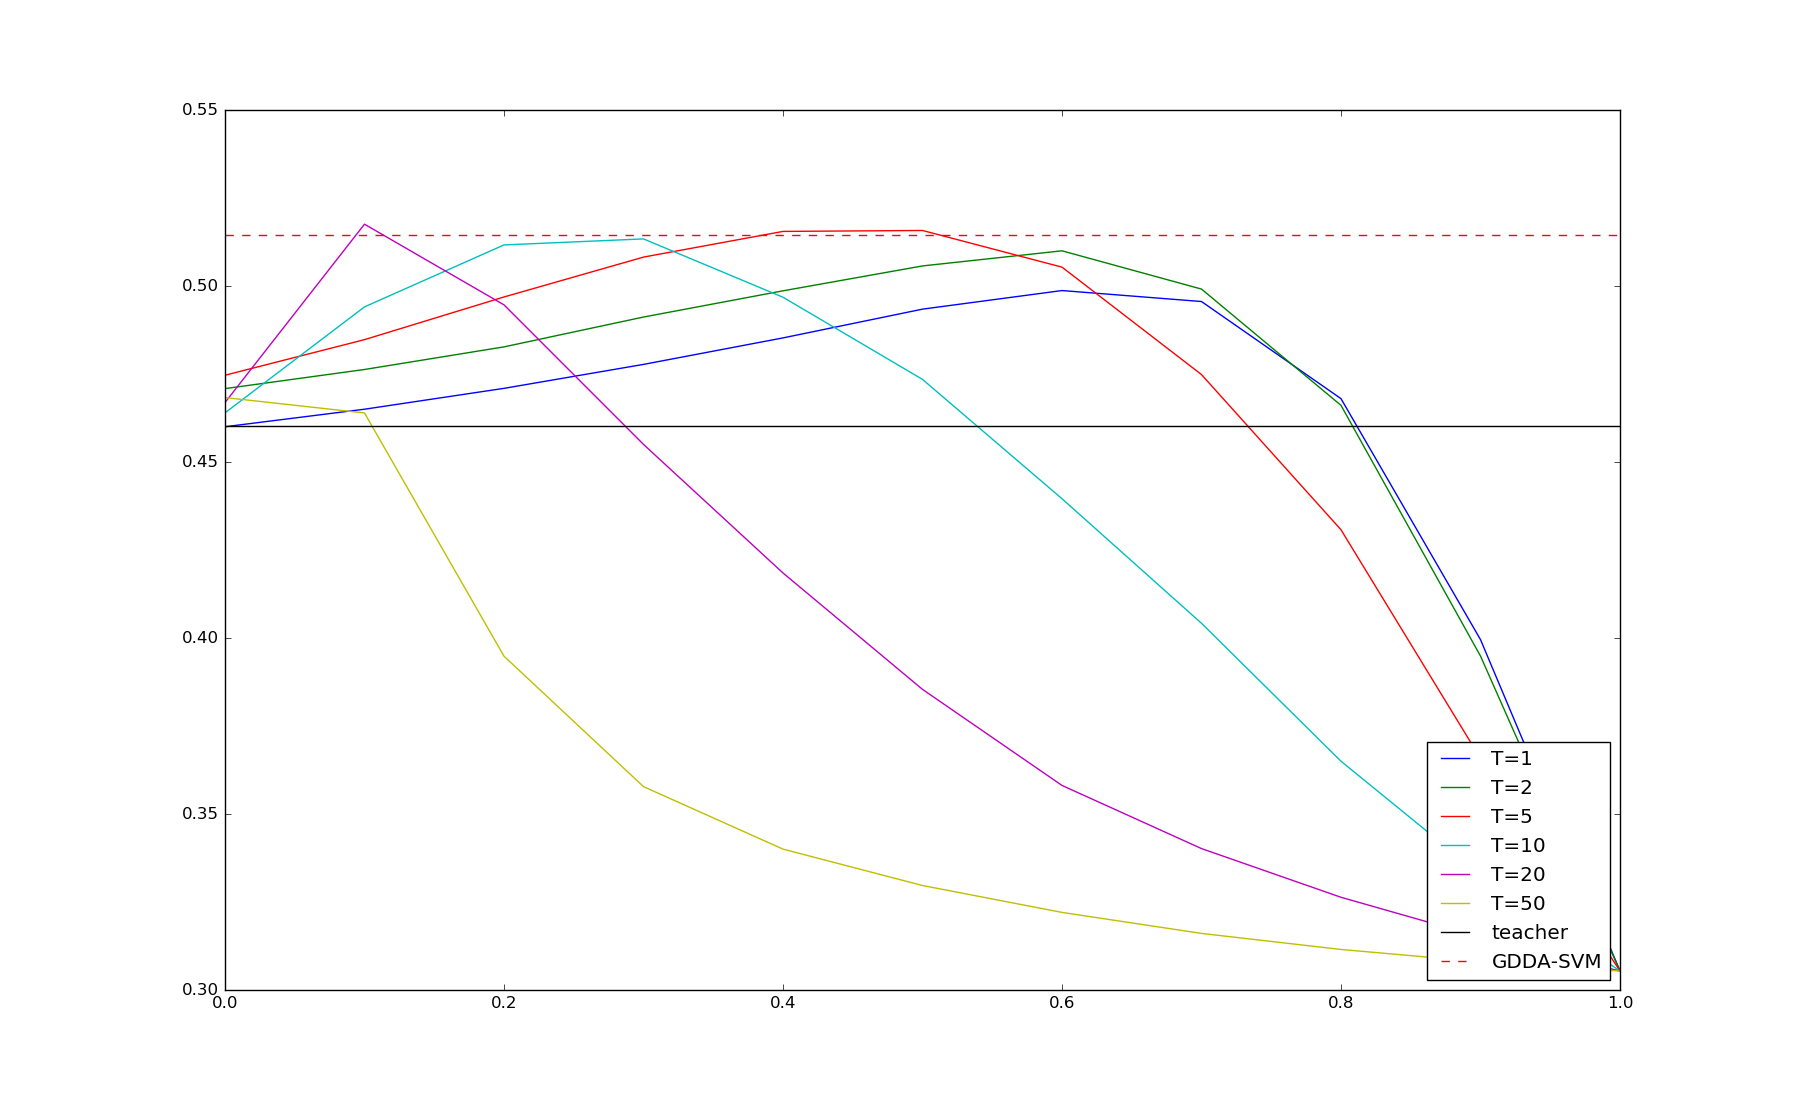
\includegraphics[width=0.45\textwidth]{figure/dslr1.png}}&
\subfloat[10 unlabeled]{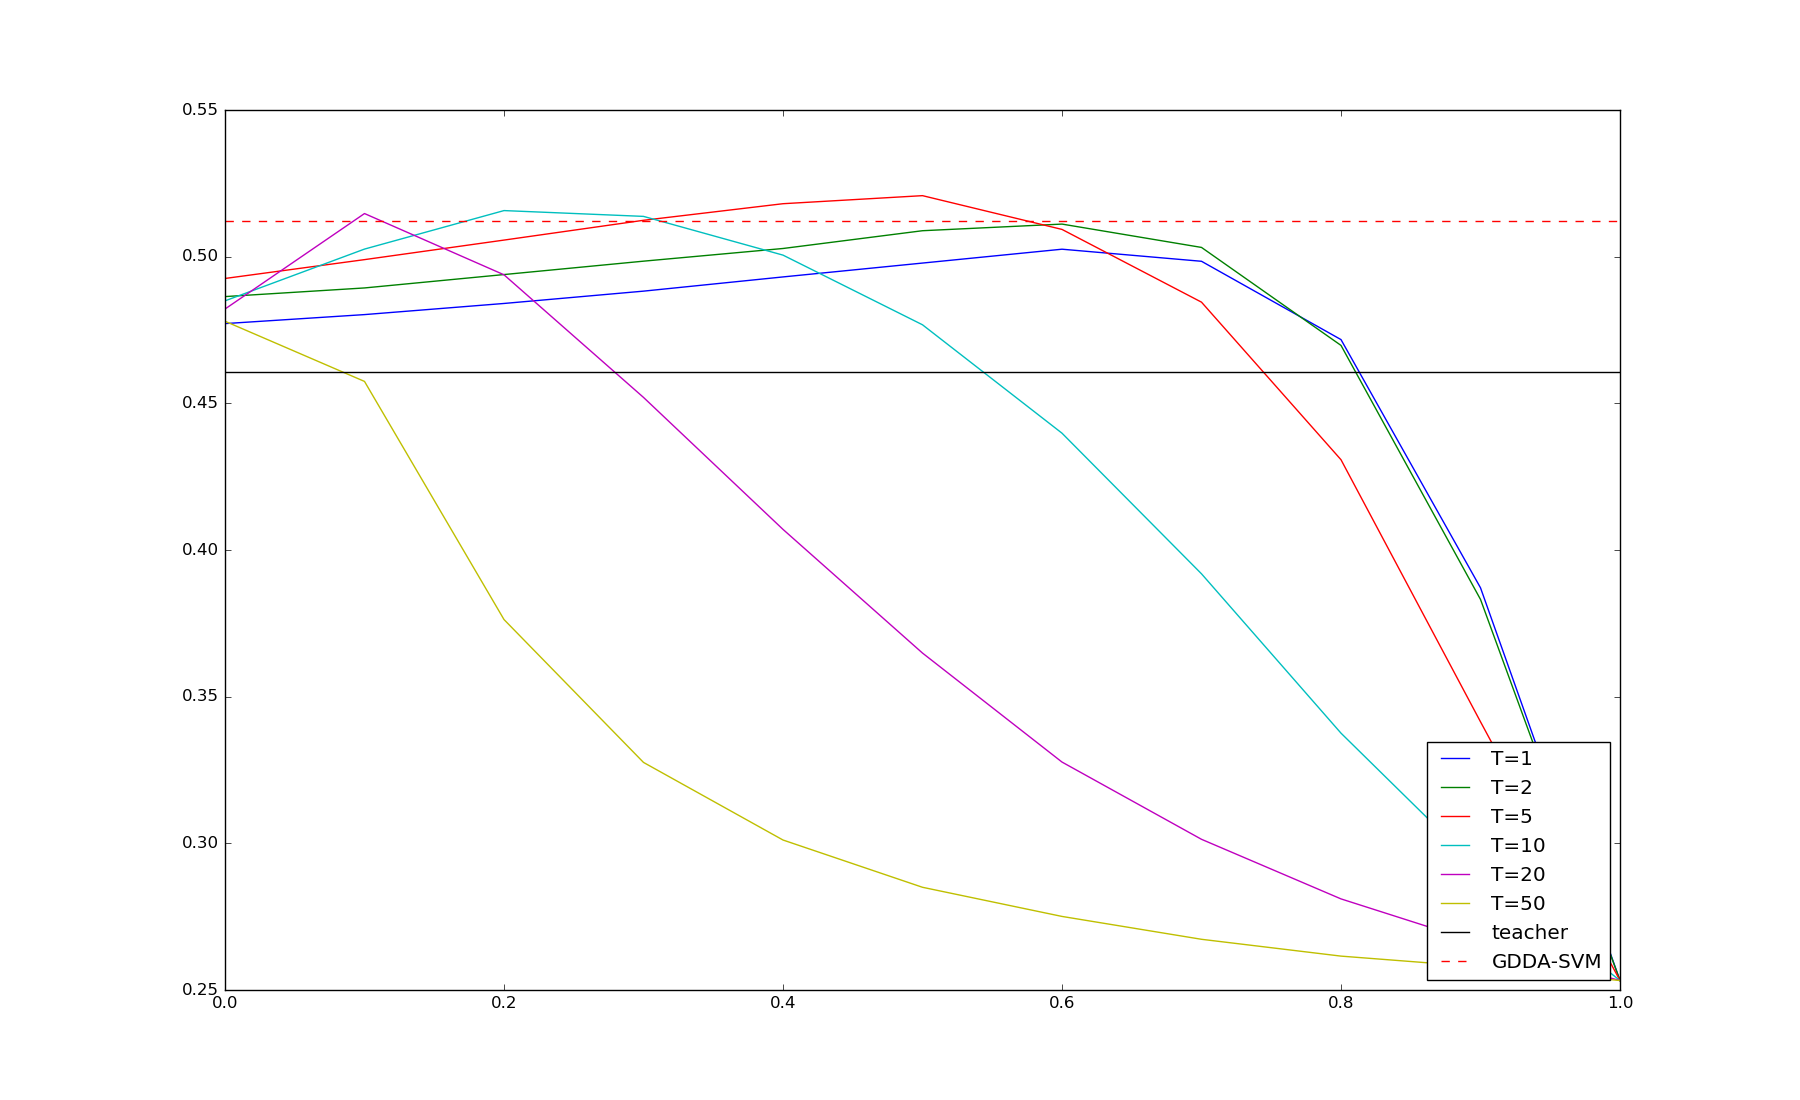
\includegraphics[width=0.45\textwidth]{figure/dslr2.png}}\\
\subfloat[15 unlabeled]{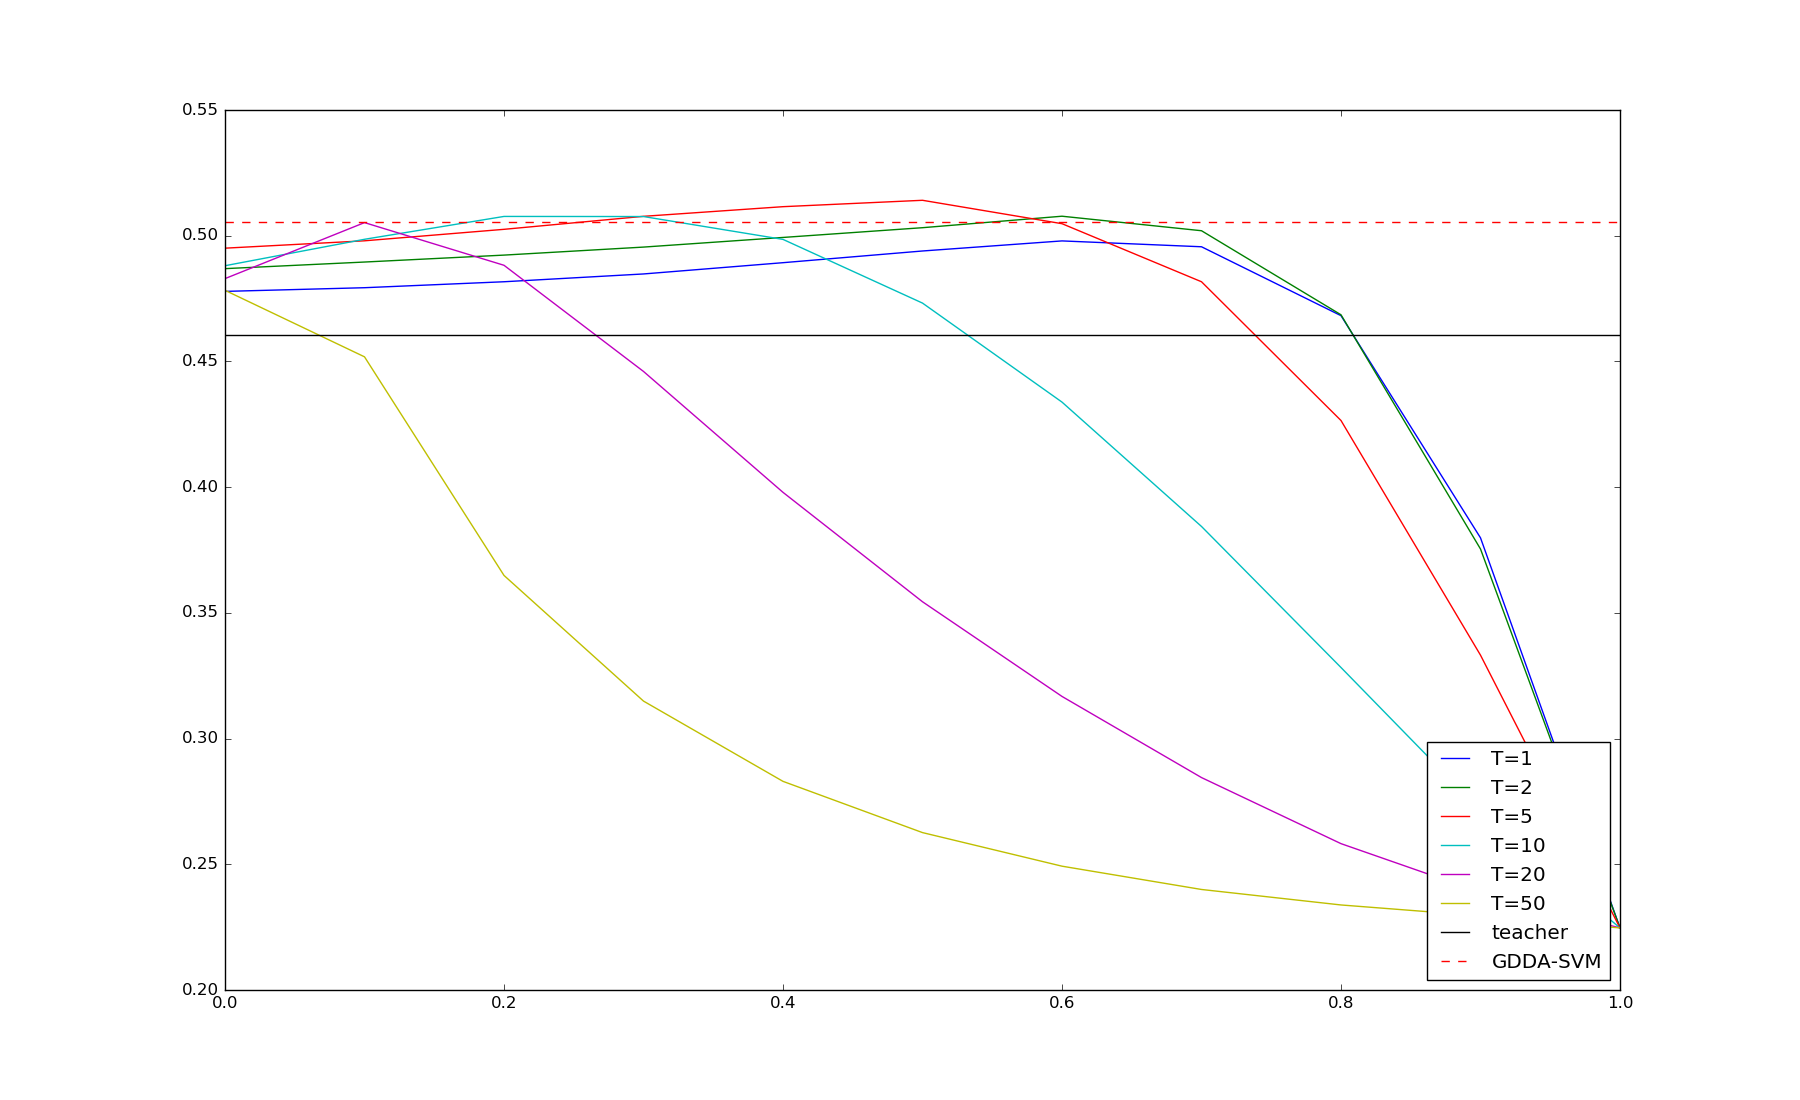
\includegraphics[width=0.45\textwidth]{figure/dslr3.png}}&
\subfloat[20 unlabeled]{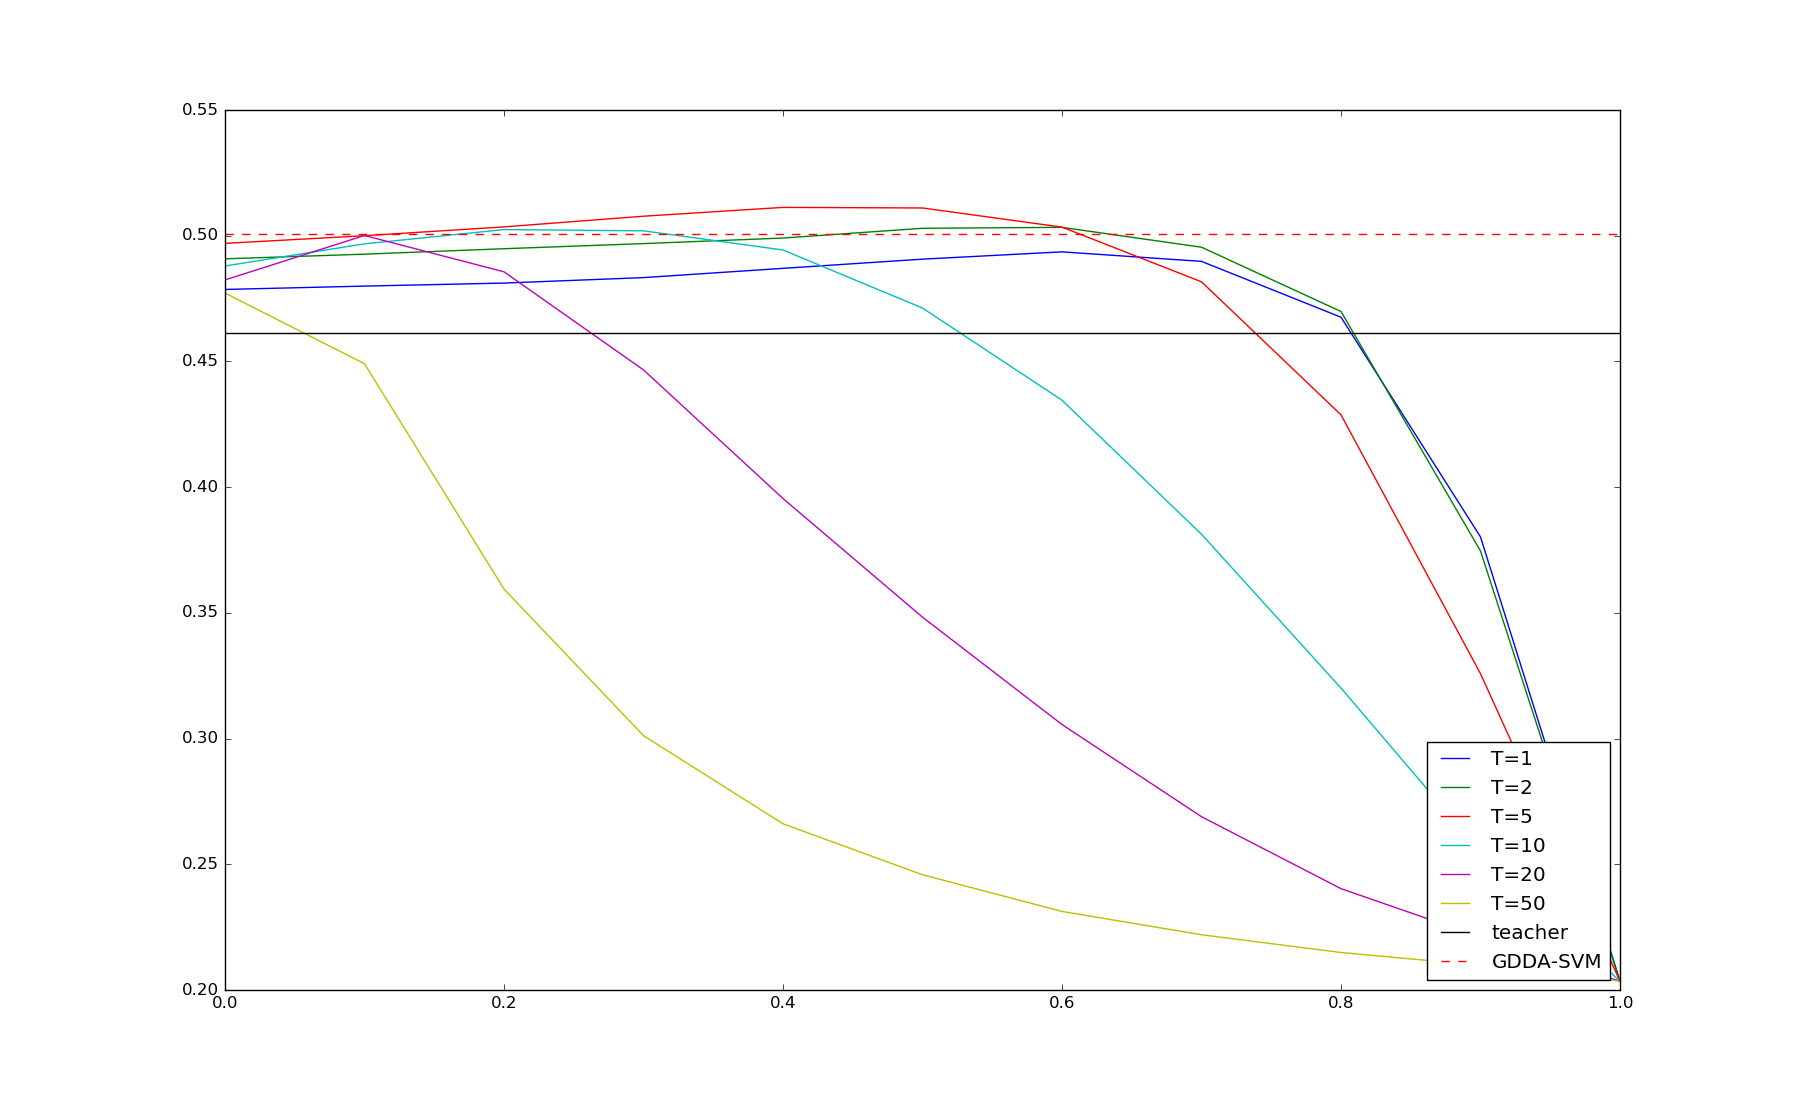
\includegraphics[width=0.45\textwidth]{figure/dslr4.png}}\\
\end{tabular}
\caption{DSLR $\rightarrow$ Amazon. Semi-supervised adaptation with one labeled instance per class.}\label{fig:single1}
\end{figure}
%\newpage
%\subsubsection{From Webcam to Amazon}
\begin{figure}[h]
\centering
\begin{tabular}{cc}
\subfloat[5 unlabeled ]{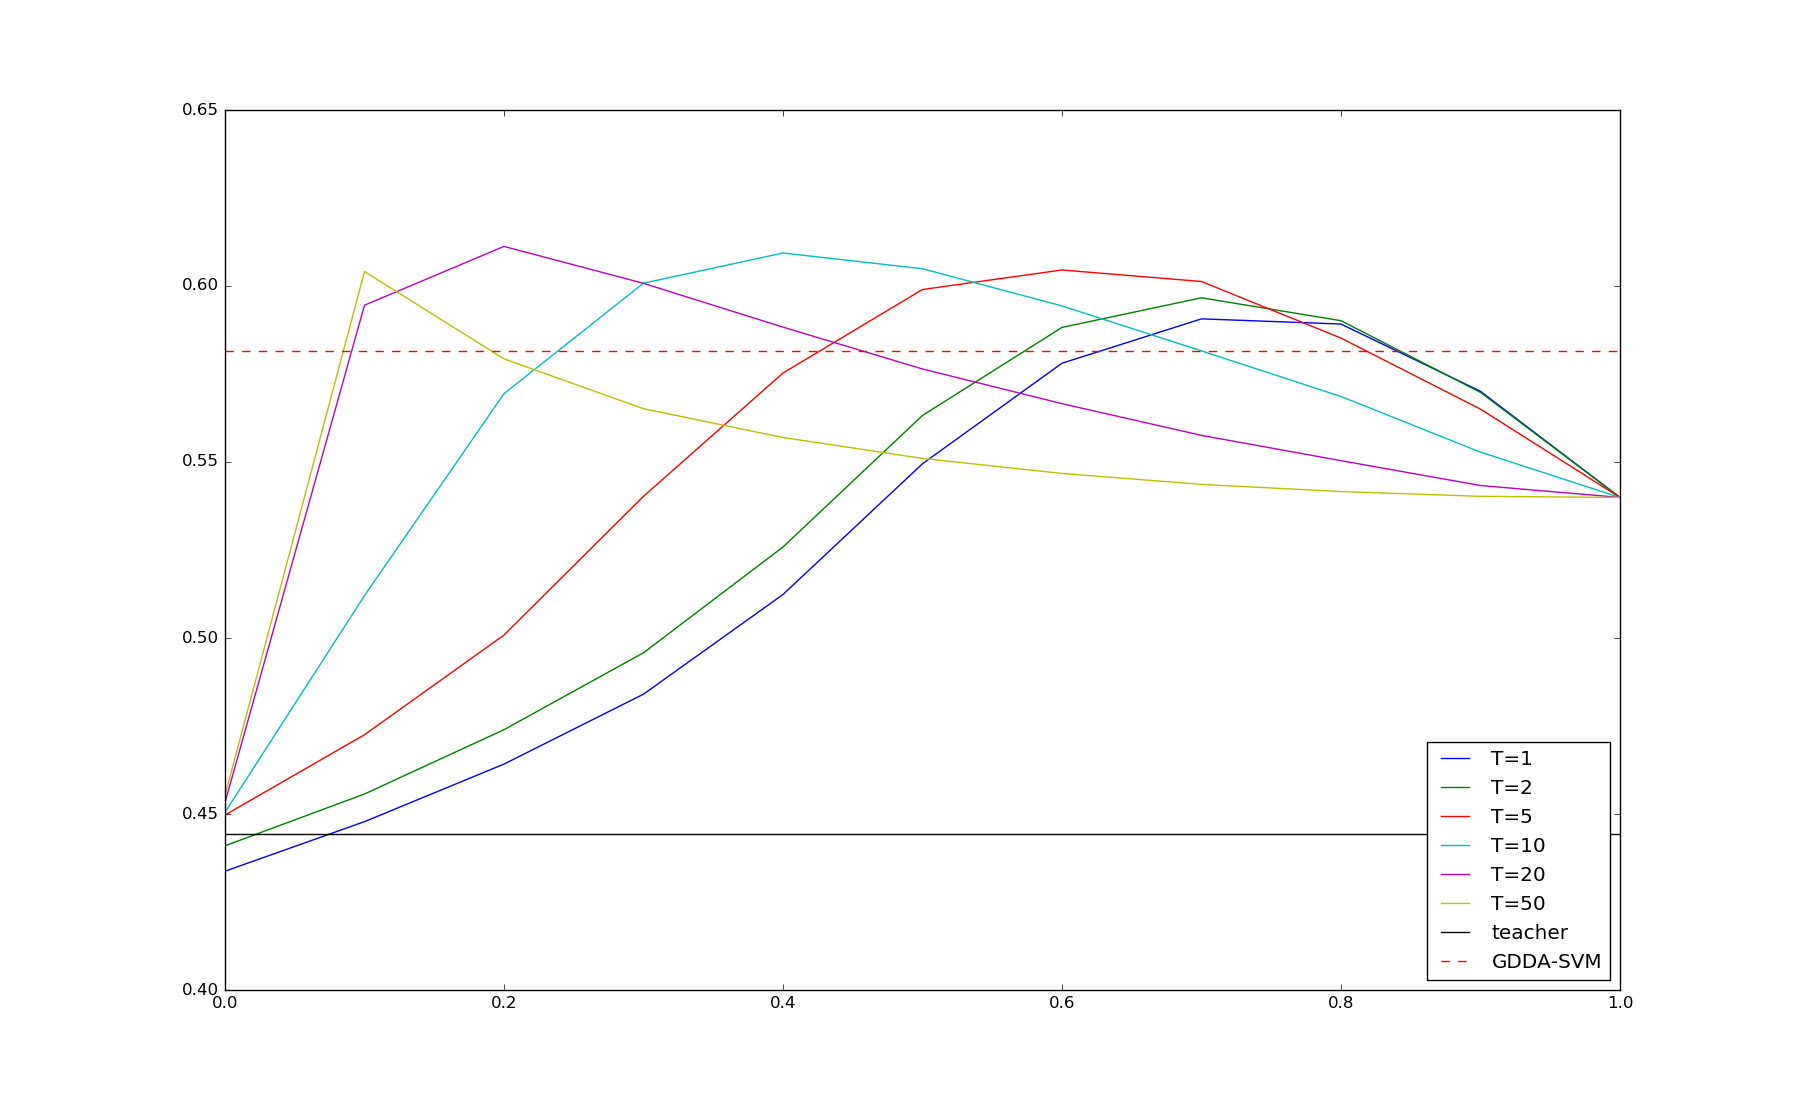
\includegraphics[width=0.45\textwidth]{figure/webcam1.png}}&
\subfloat[10 unlabeled]{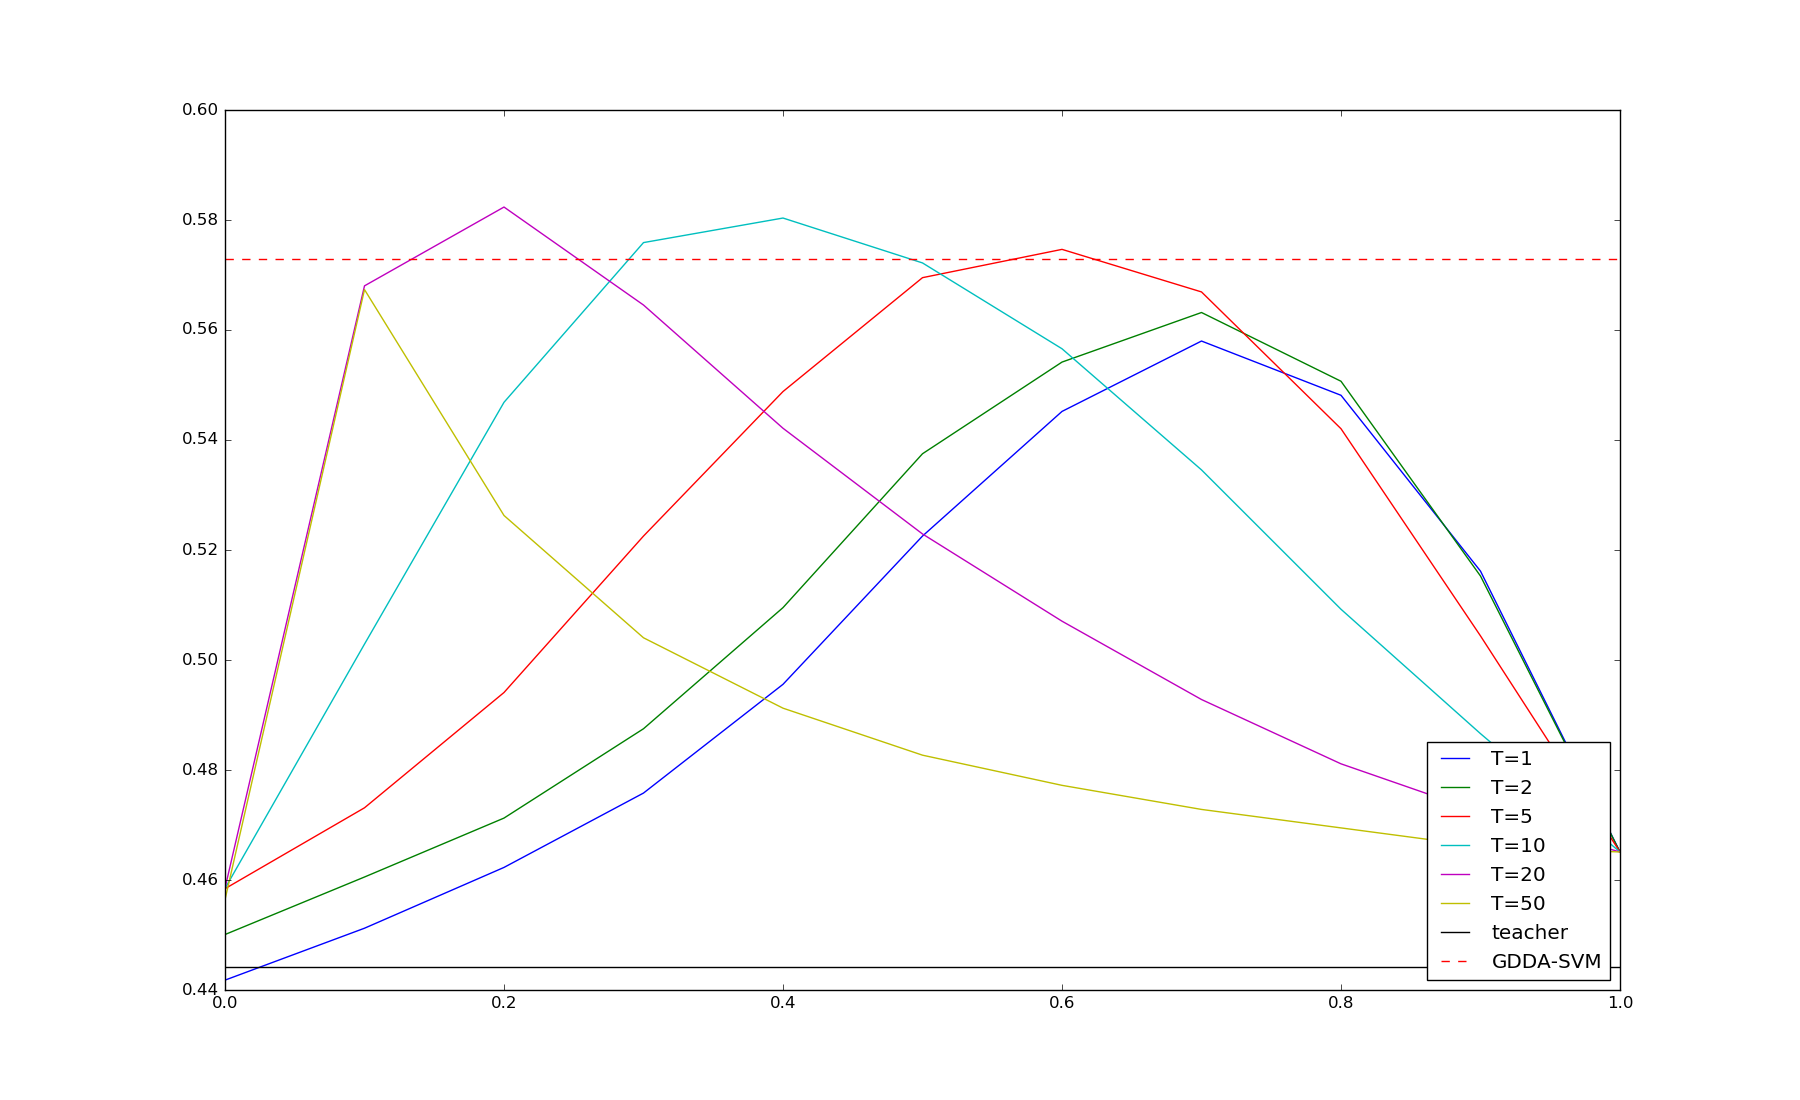
\includegraphics[width=0.45\textwidth]{figure/webcam2.png}}\\
\subfloat[15 unlabeled]{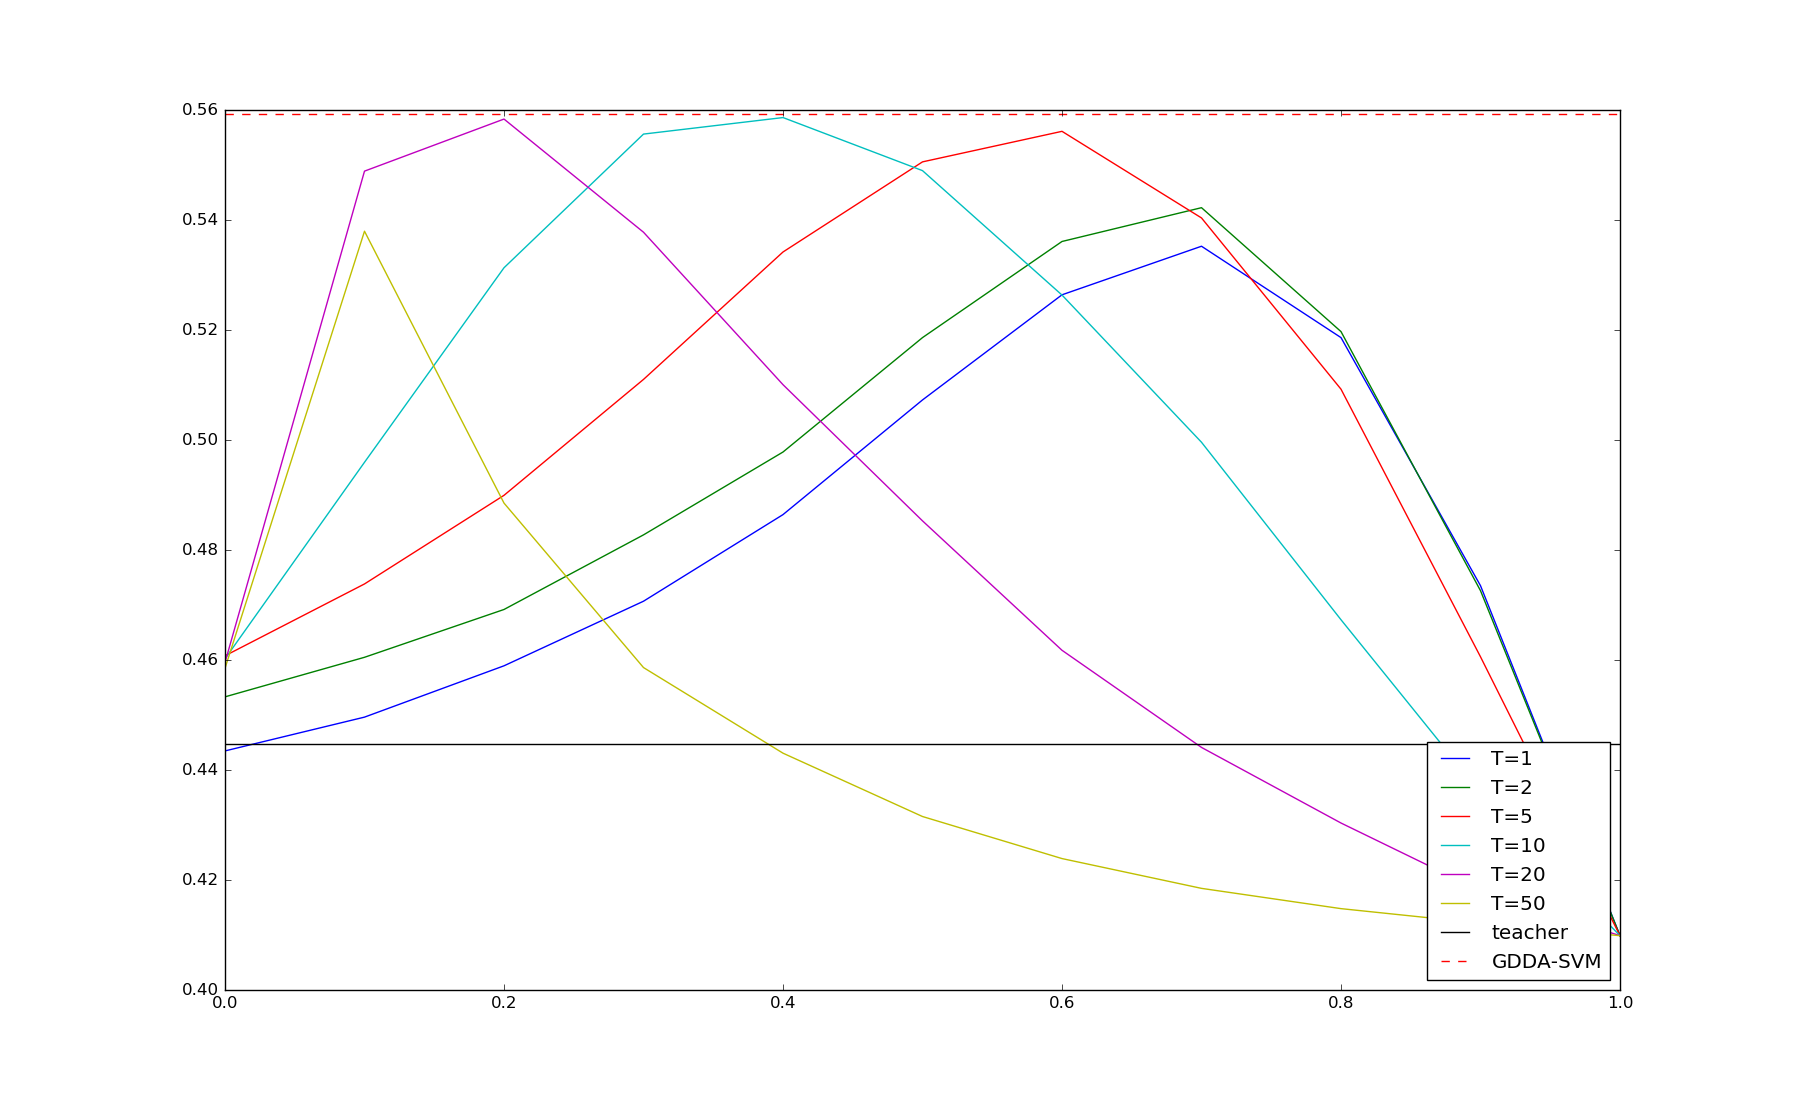
\includegraphics[width=0.45\textwidth]{figure/webcam3.png}}&
\subfloat[20 unlabeled]{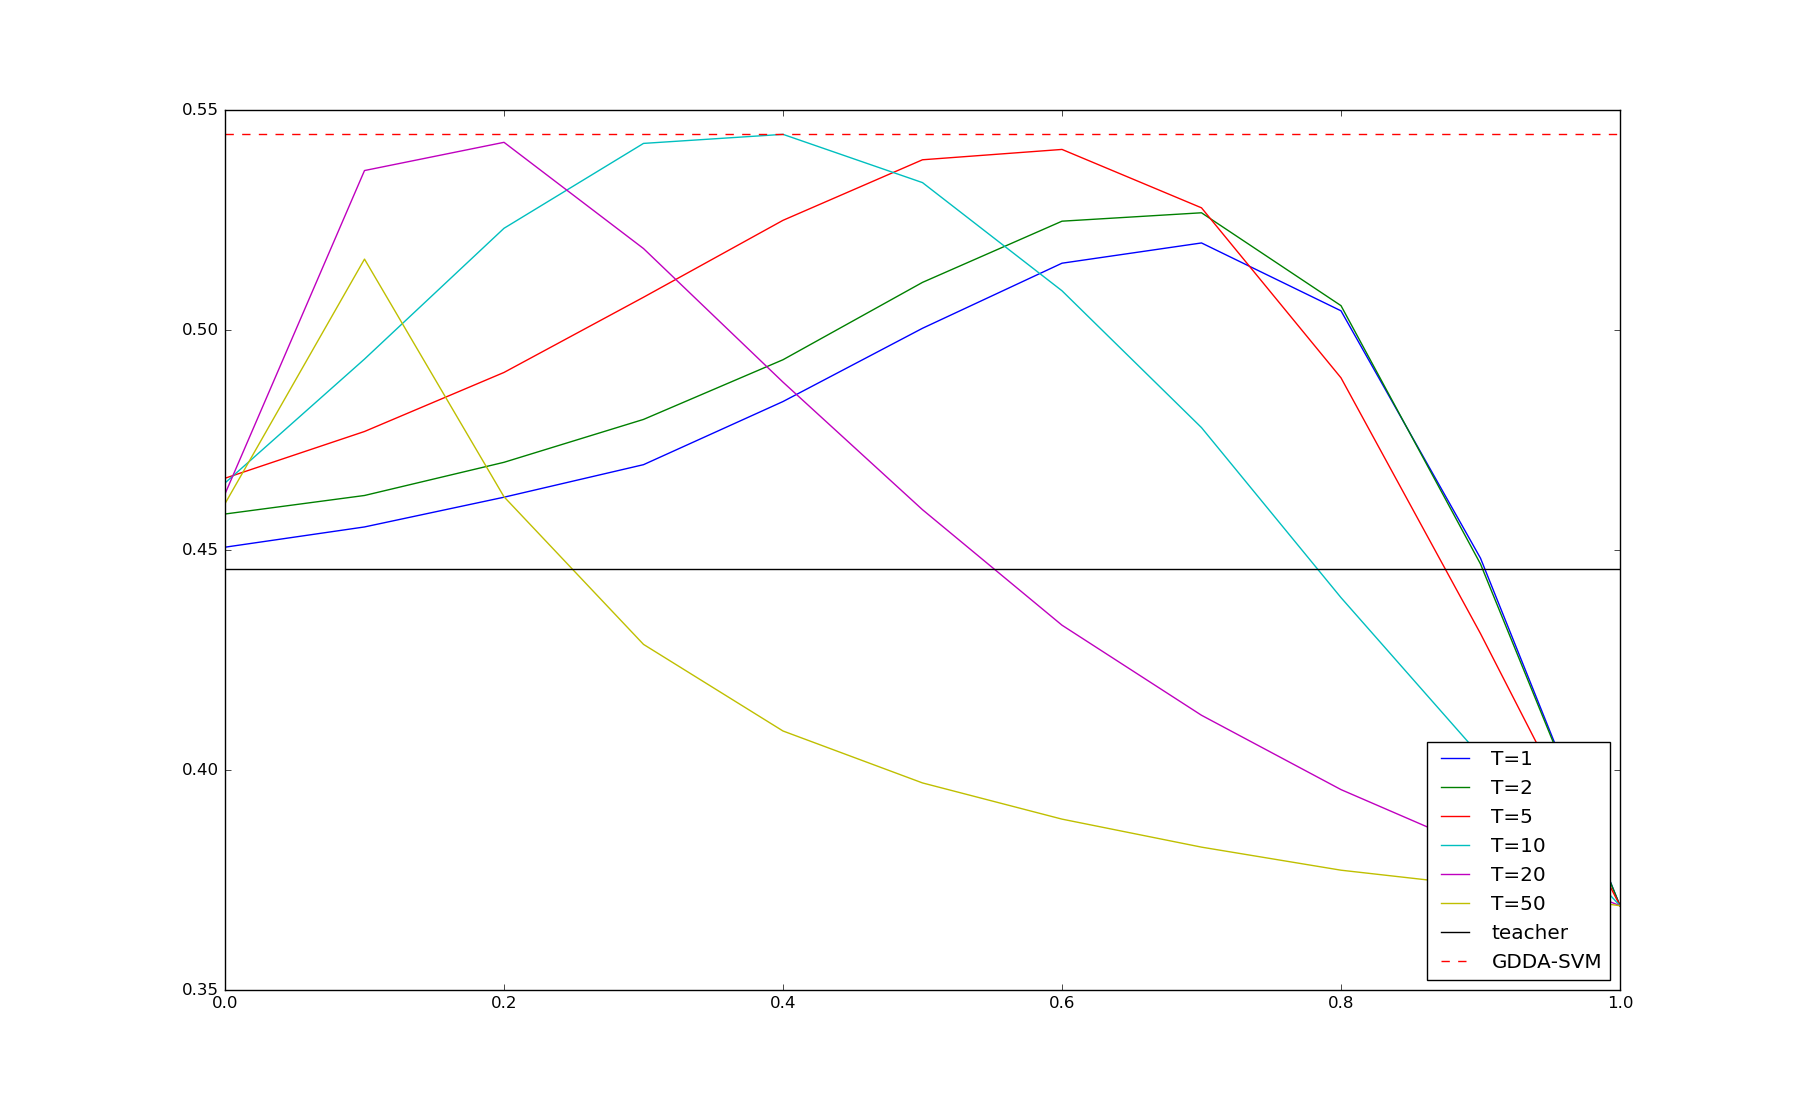
\includegraphics[width=0.45\textwidth]{figure/webcam4.png}}\\
\end{tabular}
\caption{Webcam $\rightarrow$ Amazon. Semi-supervised adaptation with one labeled instance per class.}\label{fig:single2}
\end{figure}
\subsection{Multi-Source for Office datasets}
We transfer DSLR and Webcam to Amazon datasets with different settings similar to the experiment above. The experiment results are shown in Figure \ref{fig:multi}. In our experiment we have two baselines the source models from DSLR and Webcam (denoted as teacher 1 and teacher 2). We also show the performance of GDDA-SVM with each of the single source model (denoted as GDDA-SVM1 and GDDA-SVM2).
The performance of the 2-source GDDA-SVM is denoted as GDDA-SVM-Multi.


\textbf{Observation:} The GDDA-SVM-Multi can exploit the knowledge from both source models effectively and outperform any single source model as well as the source models themselves.
\begin{figure}[h]
\centering
\begin{tabular}{cc}
\subfloat[5 unlabeled ]{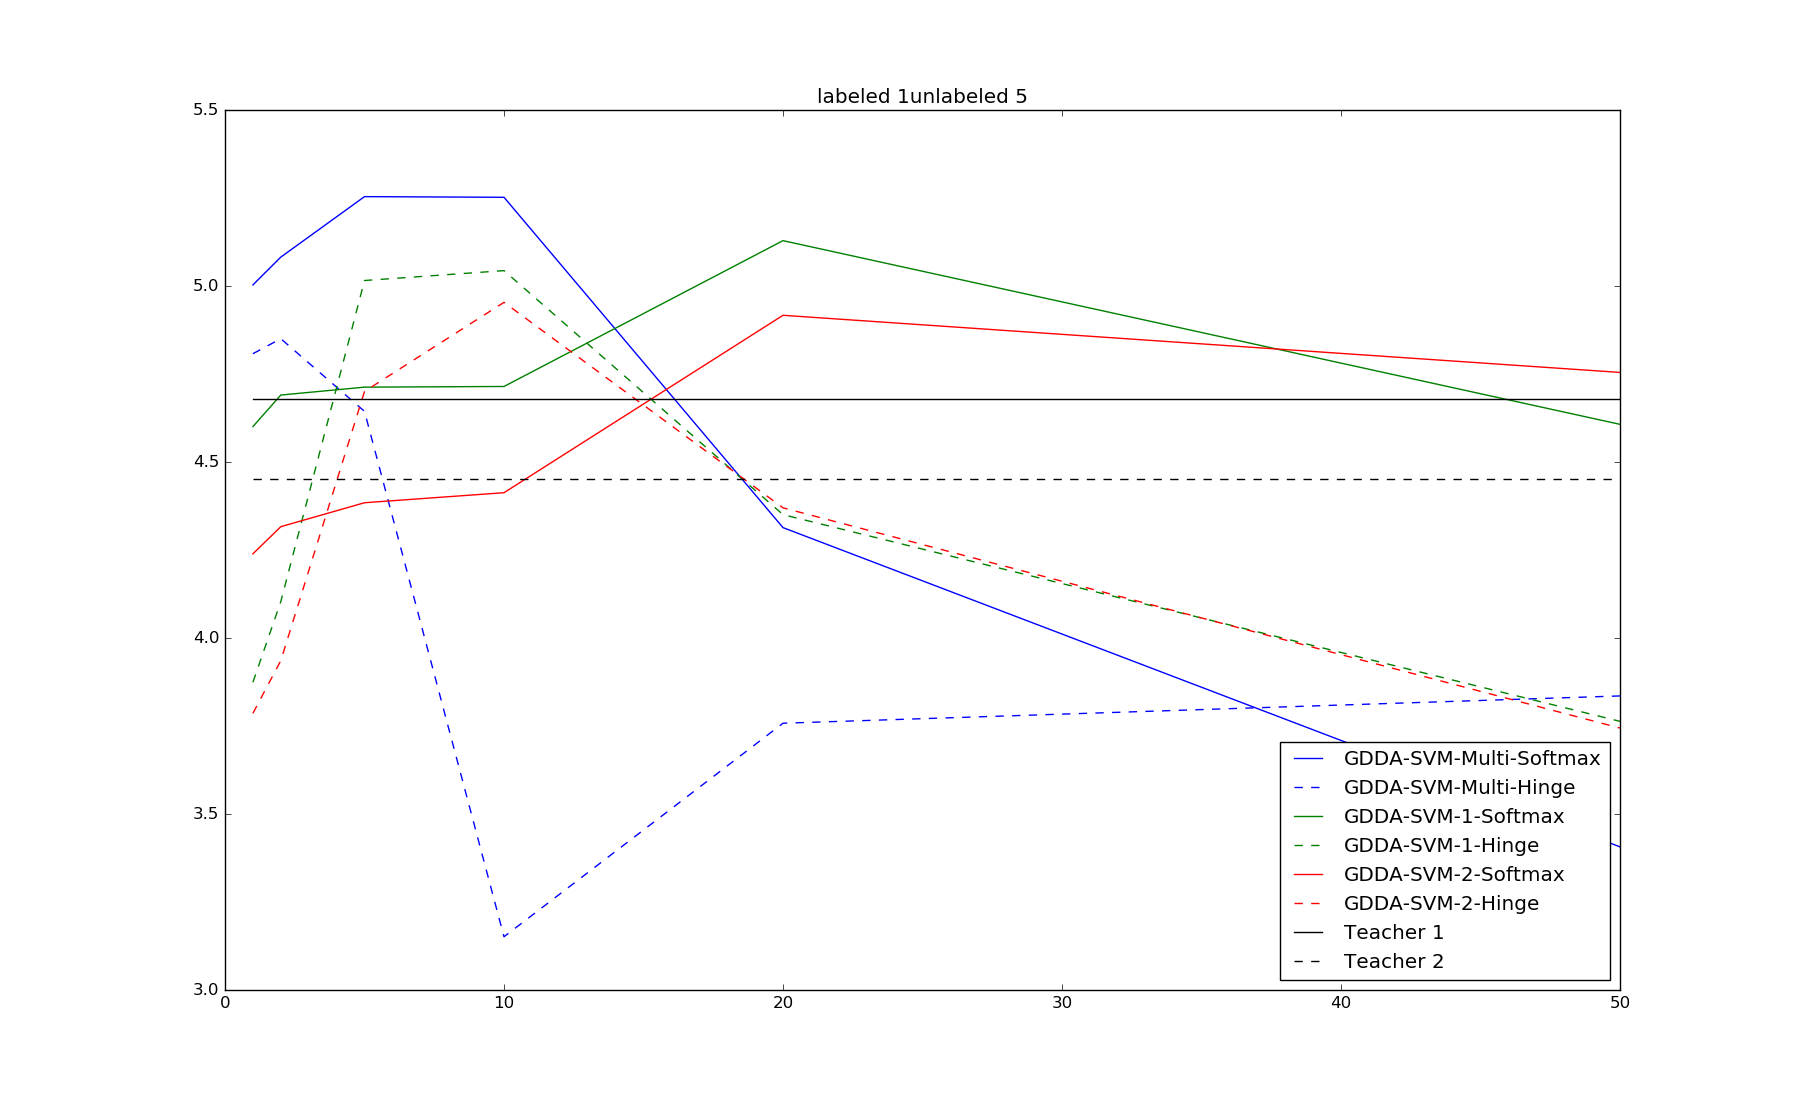
\includegraphics[width=0.45\textwidth]{figure/labeled1 unlabeled5.png}}&
\subfloat[10 unlabeled]{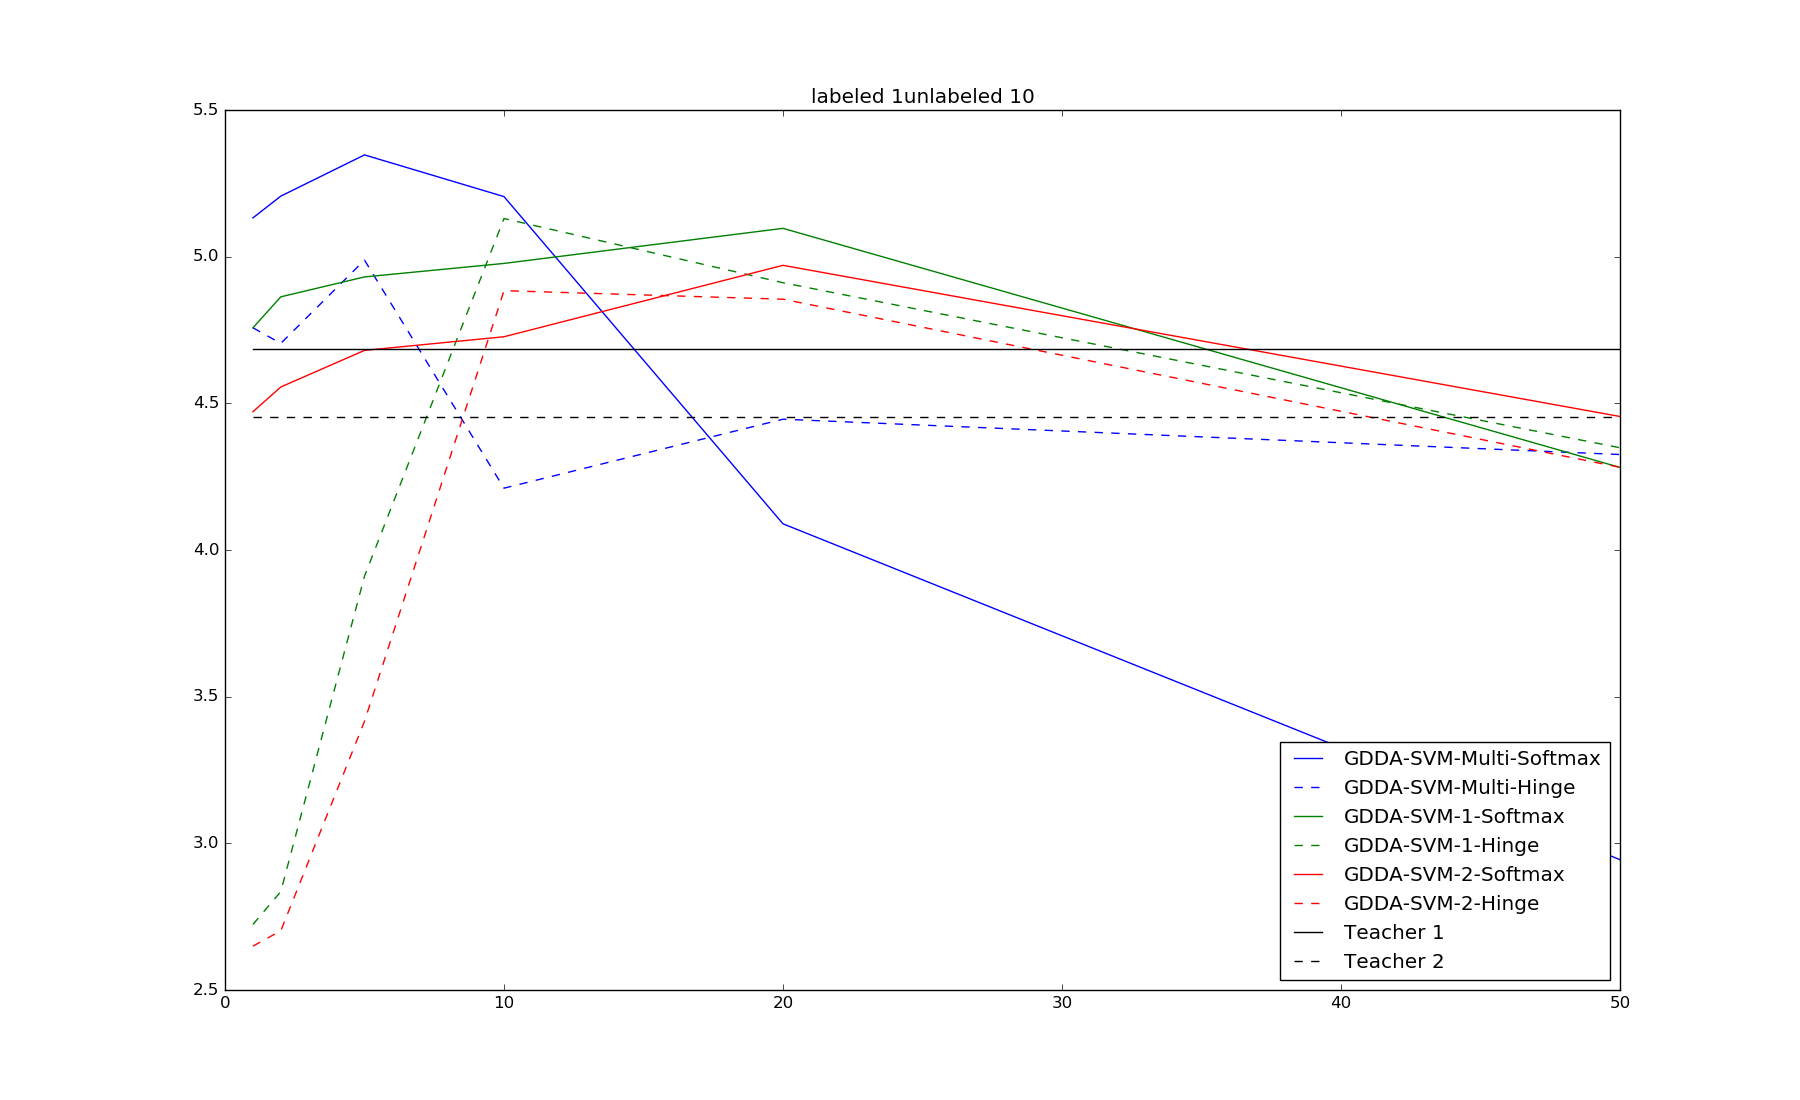
\includegraphics[width=0.45\textwidth]{figure/labeled1 unlabeled10.png}}\\
\subfloat[15 unlabeled]{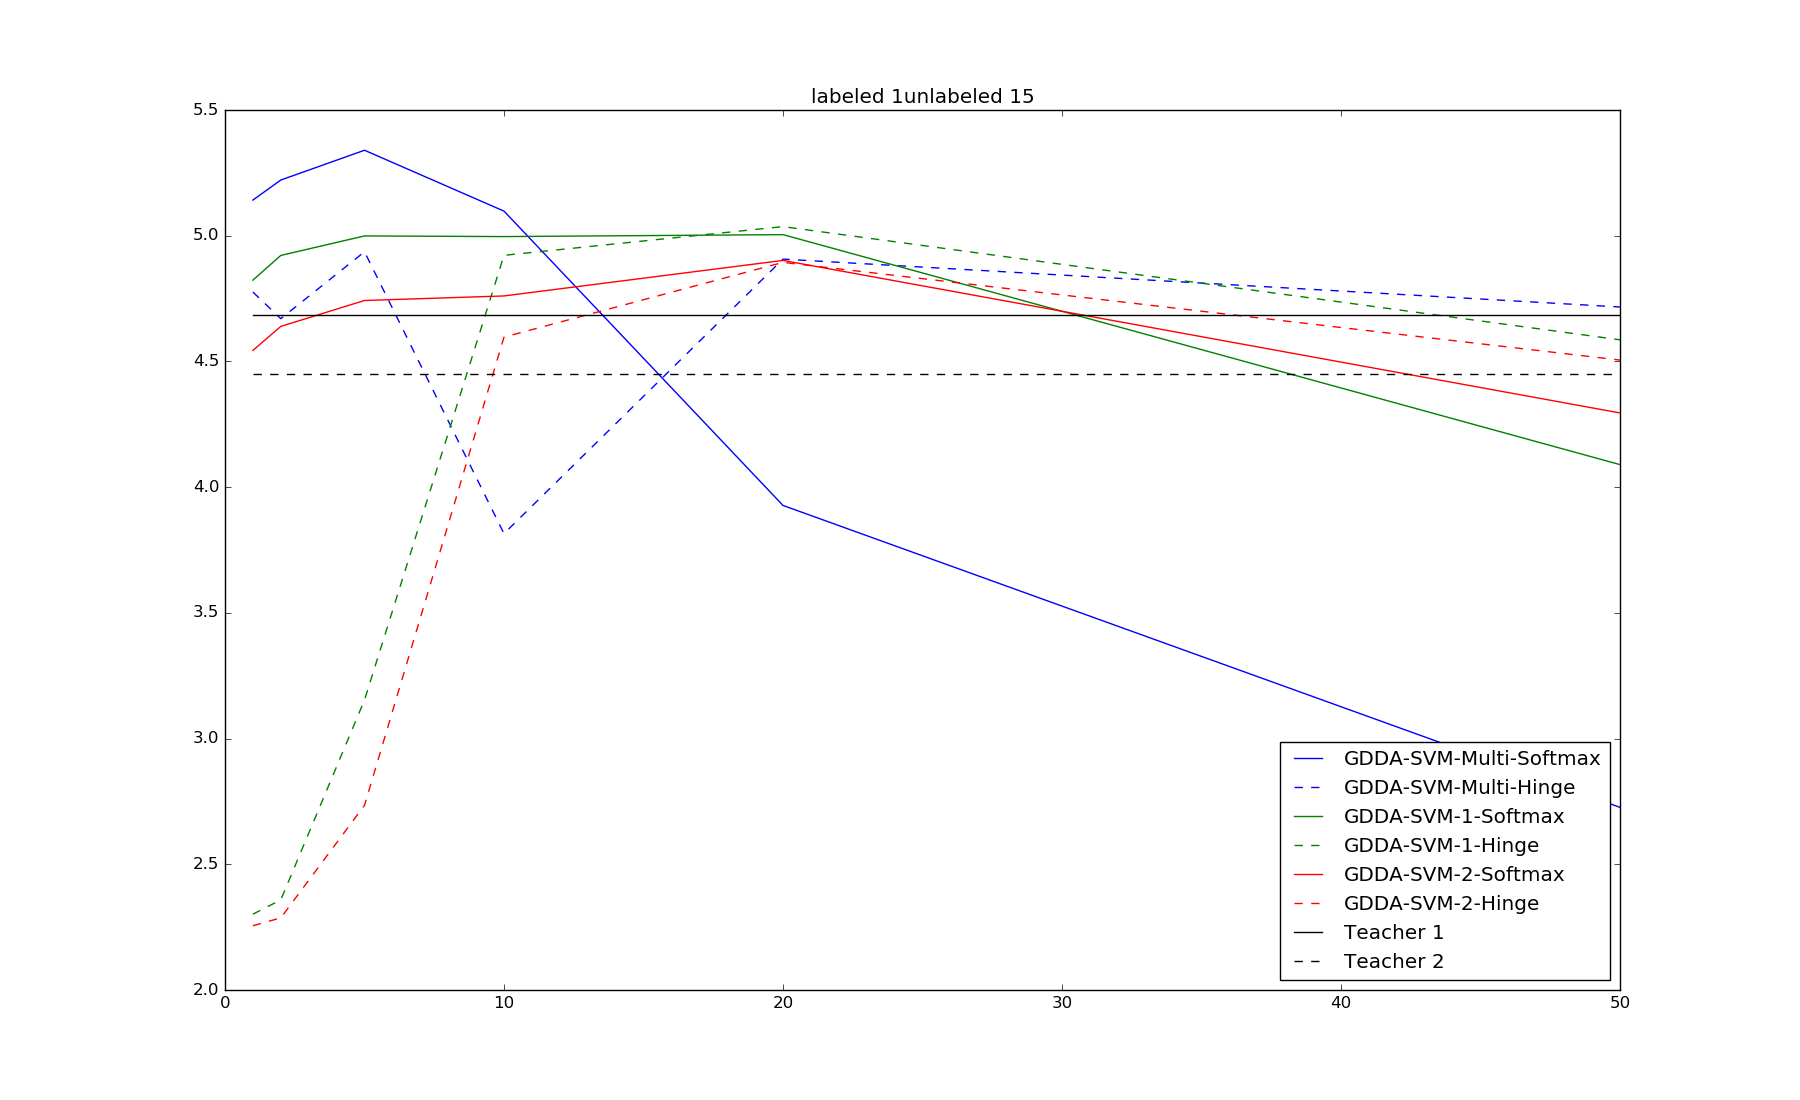
\includegraphics[width=0.45\textwidth]{figure/labeled1 unlabeled15.png}}&
\subfloat[20 unlabeled]{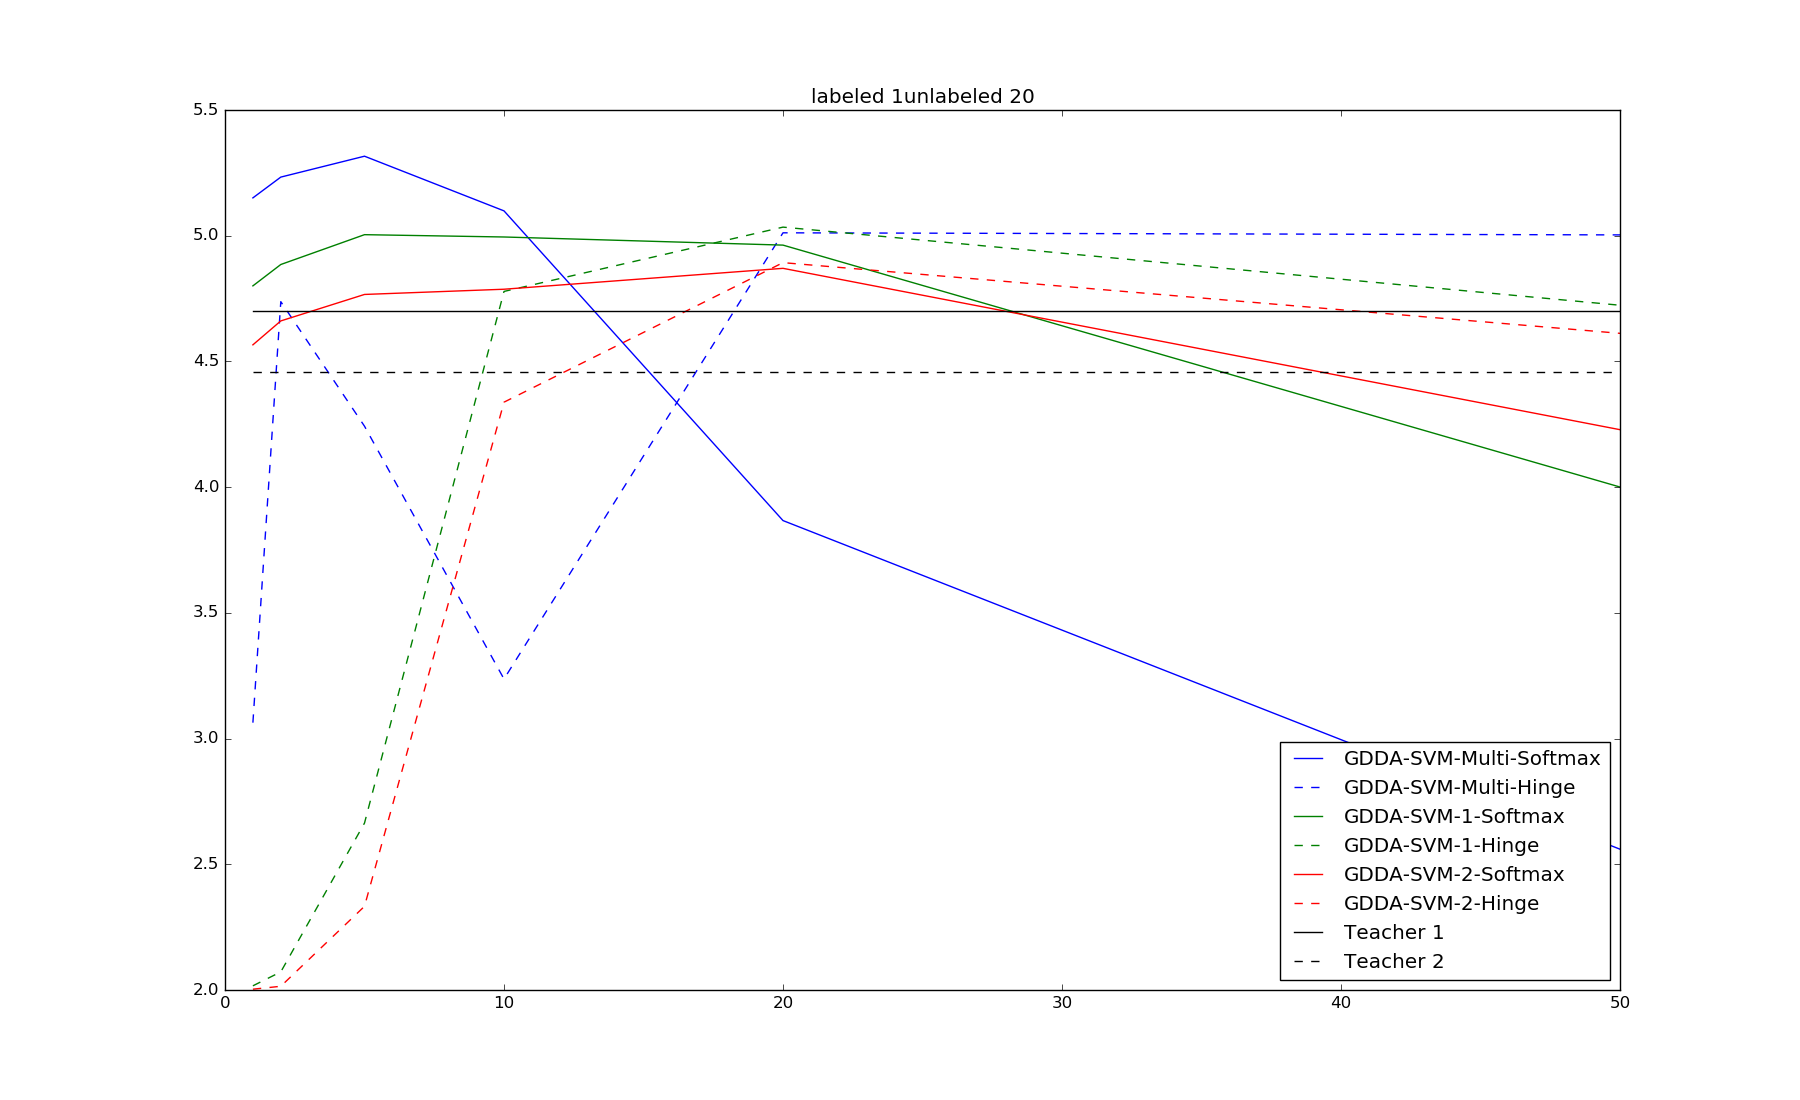
\includegraphics[width=0.45\textwidth]{figure/labeled1 unlabeled20.png}}\\
\end{tabular}
\caption{Webcam $\rightarrow$ Amazon. Semi-supervised adaptation with one labeled instance per class.}\label{fig:multi}
\end{figure}


